% ------------------------------------------------------------------------
% Senac Tex: Modelo de Trabalho Academico para o Centro Universitário
% Senac
% ------------------------------------------------------------------------

% ========================================================================
% CONFIGURAÇÃO DO DOCUMENTO
% ========================================================================


\documentclass[
	% -- opções da classe memoir --
	12pt,				% tamanho da fonte
	openright,			% capítulos começam em pág ímpar (insere página vazia caso preciso)
	oneside,			% para impressão em verso e anverso. Oposto a oneside
	a4paper,			% tamanho do papel. 
	% -- opções da classe abntex2 --
	%chapter=TITLE,		% títulos de capítulos convertidos em letras maiúsculas
	%section=TITLE,		% títulos de seções convertidos em letras maiúsculas
	%subsection=TITLE,	% títulos de subseções convertidos em letras maiúsculas
	%subsubsection=TITLE,% títulos de subsubseções convertidos em letras maiúsculas
	% -- opções do pacote babel --
	english,			% idioma adicional para hifenização
	brazil				% o último idioma é o principal do documento
	]{abntex2}

% ---
% Pacotes básicos 
% ---
\usepackage{lmodern}			% Usa a fonte Latin Modern			
\usepackage[T1]{fontenc}		% Selecao de codigos de fonte.
\usepackage[utf8]{inputenc}		% Codificacao do documento (conversão automática dos acentos)
\usepackage{lastpage}			% Usado pela Ficha catalográfica
\usepackage{indentfirst}		% Indenta o primeiro parágrafo de cada seção.
\usepackage{color}				% Controle das cores
\usepackage{graphicx}			% Inclusão de gráficos
\usepackage{microtype} 			% para melhorias de justificação
\usepackage{listings}
\usepackage{indentfirst}
\usepackage[top=3cm, bottom=2cm, left=3cm, right=2cm]{geometry}

% ---
% Pacotes de citações
% ---
\usepackage[brazilian,hyperpageref]{backref}	 % Paginas com as citações na bibl
\usepackage[alf]{abntex2cite}	% Citações padrão ABNT

% CONFIGURAÇÕES DE PACOTES

% Configurações do pacote backref
% Usado sem a opção hyperpageref de backref
\renewcommand{\backrefpagesname}{Citado na(s) página(s):~}
% Texto padrão antes do número das páginas
\renewcommand{\backref}{}
% Define os textos da citação
\renewcommand*{\backrefalt}[4]{
	\ifcase #1 %
		Nenhuma citação no texto.%
	\or
		Citado na página #2.%
	\else
		Citado #1 vezes nas páginas #2.%
	\fi}%

% Informações de dados para CAPA e FOLHA DE ROSTO
\titulo{Titulo do Trabalho}
\autor{Lucas da Mata Guimarães}
\local{São Paulo - Brasil}
\data{2025}
\orientador{Nome do Orientador}
%\coorientador{Nome do Coorientador}
\instituicao{
  Centro Universitário Senac - Santo Amaro
  \par
  Bacharelado em Ciência da Computação
}
\tipotrabalho{Trabalho de Conclusão de Curso}
% O preambulo deve conter o tipo do trabalho, o objetivo, 
% o nome da instituição e a área de concentração 
\preambulo{Monografia apresentada na disciplina Trabalho de Conclusão de Curso, como parte dos requisitos para obtenção do título de Bacharel em Ciência da Computação.}

% Configurações de aparência do PDF final

% alterando o aspecto da cor azul
\definecolor{blue}{RGB}{41,5,195}

% informações do PDF
\makeatletter
\hypersetup{
     	%pagebackref=true,
		pdftitle={\@title}, 
		pdfauthor={\@author},
    	pdfsubject={\imprimirpreambulo},
	    pdfcreator={LaTeX with abnTeX2},
		pdfkeywords={abnt}{latex}{abntex}{abntex2}{trabalho acadêmico}, 
		colorlinks=true,       		% false: boxed links; true: colored links
    	linkcolor=blue,          	% color of internal links
    	citecolor=blue,        		% color of links to bibliography
    	filecolor=magenta,      		% color of file links
		urlcolor=blue,
		bookmarksdepth=4
}
\makeatother

% Espaçamentos entre linhas e parágrafos 

% O tamanho do parágrafo é dado por:
\setlength{\parindent}{1.25cm}

% Controle do espaçamento entre um parágrafo e outro:
\setlength{\parskip}{0.2cm}

\SingleSpacing
\makeatletter
\let\@fnsymbol\@arabic
\makeatother

% compila o indice
\makeindex

\begin{document}

% Retira espaço extra obsoleto entre as frases.
\frenchspacing

% ========================================================================
% CAPA
% ========================================================================
\imprimircapa

% ========================================================================
% FOLHA DE ROSTO
% ========================================================================
\imprimirfolhaderosto

% ========================================================================
% DEDICATÓRIA
% ========================================================================
 \begin{dedicatoria}
   \vspace*{\fill}
   \centering
   \noindent
   \textit{ Texto da dedicatória.} \vspace*{\fill}
 \end{dedicatoria}

% ========================================================================
% AGRADECIMENTOS
% ========================================================================
 \begin{agradecimentos}
 Texto de agradecimento.

 \end{agradecimentos}

% ========================================================================
% EPÍGRAFE
% ========================================================================
 \begin{epigrafe}
     \vspace*{\fill}
 	\begin{flushright}
 		\textit{``A vingança nunca é plena, \\
 		mata a alma e a envenena. \\
 		(MADRUGA, Seu, Chaves)}
 	\end{flushright}
 \end{epigrafe}

% ========================================================================
% RESUMO
% ========================================================================
\setlength{\absparsep}{18pt} % ajusta o espaçamento dos parágrafos do resumo
\begin{resumo}

Texto do resumo

\textbf{Palavras-chaves}: palavra-chave 1, palavra-chave 2, palavra-chave 3.
\end{resumo}

% ========================================================================
% ABSTRACT
% ========================================================================
\begin{resumo}[Abstract]
 \begin{otherlanguage*}{english}
    Abstract text in english
   
   \textbf{Key-words}: keyword 1, keyword 2, keyword 3
 \end{otherlanguage*}
\end{resumo}

% ========================================================================
% LISTA DE ILISTRAÇÕES
% ========================================================================
\pdfbookmark[0]{\listfigurename}{lof}
\listoffigures*
\cleardoublepage

% ========================================================================
% LISTA DE TABELAS
% ========================================================================
\pdfbookmark[0]{\listtablename}{lot}
\listoftables*
\cleardoublepage

% ========================================================================
% LISTA DE ABREVIATURAS E SIGLAS
% ========================================================================
\begin{siglas}
  \item[GAM] Generalized Additive Models
  \item[GLM] Generalized Linear Model
  \item[MARS] Multivariate Adaptive Regression Spline
  \item[ML] Maximum likelihood
\end{siglas}

% ========================================================================
% SUMÁRIO
% ========================================================================
\pdfbookmark[0]{\contentsname}{toc}
\tableofcontents*
\cleardoublepage

\textual
% ========================================================================
% INTRODUÇÃO
% ========================================================================
\chapter{Introdução}

\section{Contexto}

O uso de modelos computacionais, na Biologia, possibilita o avanço de diferentes
estudos \cite{modelagem_comp}, uma destas aplicações são os modelos de distribuição 
de especies, que são capazes de fornecer uma visualização da situação 
da fauna e flora de determinada região, podendo mostrar como estas estão se 
comportando no decorrer do tempo \cite{speciesDistributionModels}.

Entr os modelos mais utilizados estão, o Generalized Additive Models (GAM) \cite{GAM}, 
o Generalized Linear Model (GLM) \cite{GLM}, esses dois modelos usam uma função para 
estabelecer uma relação entre a média da variável de resposta e uma função 'suavizada'
das variáveis explanatórias, sendo o GLM uma estenção de modelos lineares que não
forçam o dado a escalas não naturais, e o GAM uma extenção semi-parametrizada do GLM,
tendo a capacidade de atuar com relações não lineares e não monótonas \cite{GAMeGLM_especie_estudo}. 

E o Multivariate Adaptive Regression Spline (MARS), que combina partição recursiva e ajustes
por splines, de modo a manter seus aspectos positivos, enquanto sendo menos vulneravel a 
suas propriedades não favoraveis. Gerando um conjunto de regras para prever
valores futuros apartir de uma análise regressiva. \cite{MARS} 

As implementações mais utilizadas destes são encontradas nas bibliotecas da linguagem 
R, mgcv \cite{mgcv} para GAM e GLM, e mda \cite{mda} para MARS.

Porem, estes modelos podem requisitar uma alta demanda de processamento e memória do computador hospedeiro, 
como citado por \cite{modelagem_comp}, ponto este, que não é repassado nos trabalhos referentes a análise 
ou uso dos modelos citados. Logo, mesmo com a facilidade de se adquirir um computador, tais modelos
requerem computadores de alto desempenho para serem treinados, tornando esse processo lento ou criando 
a necessidade de se alugar maquinas virtuais para está finalidade \cite{global_cloud_maketing}. 

E quando se colocam a necessidade de se manter um controle das populações de espécies, dentro ou próximo
a centros urbanos, a velocidade de preparo destes modelos se torna mais critica, já que precisamos ir des
dá coleta dos dados, ao treino e validação do modelo, e análise dos resultados obtidos.
 
\section{Justificativa}

Identificar a distribuição de espécies em um dado ambiente, em um determinado intervalo de tempo, 
é importante para termos noção de como as espécies estão respondendo a mudanças no ambiente, no aumento 
ou diminuição de outra espécie.

Uma vez que essas mudanças podem ser geradas pela ação humana, na construção civil e de infraestrutura 
\cite{impactConstruction}, conseguir estimar o impacto dessas ações é vantajoso para a preservação de espécies.

Além disso, estas abordagens aumentam as possibilidades para integrar a infraestrutura necessária, 
contribuindo para a sobrevivência de espécies que estão em níveis populacionais baixos.

Modelos estatísticos, que tem a capacidade de demonstrar estes eventos, aplicam de maneiras diferentes algumas 
linhas de abordagem. O Generalized Additive Models (GAM), Generalized Linear Model (GLM), e o 
Multivariate Adaptive Regression Spline (MARS), ambos com uma abordagem de Maximum likelihood (ML), 
variando em sua capacidade de atuar com um determinado tipo de dado e o custo levado para seu treinamento 
e utilização \cite{predPerform33models}.

Modelos que são utilizados na modelagem de distribuição de espécies necessitam de uma quantidade elevada de dados 
\cite{sampleSize}, de ocorrência e ausência, sendo os dados de ausência não necessários em todos os tipos de modelos.

Nem todas as espécies são facilmente modeláveis devido à dificuldade de coleta de dados, seja pela sua raridade ou habitat 
\cite{especiesDificies}. A colaboração de cidadãos na coleta de dados pode auxiliar na identificação de áreas prioritárias 
para pesquisa. Portanto, a identificação de bons modelos que trabalham com esses dados é vantajosa.

Dentro destes modelos, além da quantidade e tipo de dados necessários, precisamos levar em consideração, o custo necessário de 
processamento e o espaço de memória utilizado pelo mesmo, para este fim utilizamos a análise de complexidade 
e espaço \cite{introductionAlgorthms}, já que um modelo mais barato nesse quesito pode ser criado em computadores 
mais acessíveis \cite{introductionAnalysis}, e ser possível a construção de mais de um modelo de modo simultâneo.

Os pontos levantados anteriormente podem afetar a acurácia de um modelo, mesmo atendendo os requisitos, 
de pouco adianta se o mesmo nos entrega respostas que induzem ao erro. Identificar um modelo que tenham uma boa acurácia, 
quando trabalham somente com dados de ocorrência, assim como uma melhor avaliação computacional, se vê vantajoso para 
situações em que queremos criar uma análise inicial de um determinado senário.

\section{Objetivo}

Este trabalho tem como o bjetivo avaliar e comparar a implementação encontrada nas bibliotecas mda e mgcv da linguagem R, dos modelos
de distribuiçção de espécies, GAM, GML e MARS, levantando o custo computacional de cada um destes apartir de uma análise de 
complexidade e espaço. Encontrando um modelo que melhor aprensente um equilibrio entre a acurácia e o custo computacional.

\subsection{Objetivos Específicos}

\begin{enumerate}
	\item Análise de complexidade e espaço dos modelos.
	\begin{itemize}
		\item Generalized Addtive Model;
		\item Generalized Linear Model;
		\item Multivariate Adaptive Regression Spline;
	\end{itemize}
	\item Avaliação da acurácia dos modelos com dados de ocorrência.
	\item Comparação dos modelos.
	\item Avaliação dos modelos com base na relação custo x acurácia.
\end{enumerate}

% ========================================================================
% REVISÃO BIBLIOGRÁFICA
% ========================================================================

\chapter{Revisão Bibliográfica}

Texto de introdução do capítulo de Revisão Bibliográfica

\section{Seção do capitulo de revisão bibliográfica}
Lorem ipsum dolor sit amet, consectetur adipiscing elit. Sed sollicitudin tempor sapien in maximus. Quisque in vulputate dui, ac vestibulum sem. Suspendisse urna velit, dapibus nec egestas a, rhoncus vitae neque. Mauris quis efficitur augue. Aliquam quis tellus eget orci aliquet aliquam. Sed luctus, quam vitae elementum malesuada, quam lacus imperdiet urna, sed ullamcorper libero magna non elit. Cras laoreet arcu a augue volutpat, suscipit pretium tellus tempus. Sed eros tortor, imperdiet eu neque id, interdum egestas tortor. \cite{citacao1}

\subsection{Subseção do capítulo de Revisão Bibliográfica}

Lorem ipsum dolor sit amet, consectetur adipiscing elit. Sed sollicitudin tempor sapien in maximus. Quisque in vulputate dui, ac vestibulum sem. Suspendisse urna velit, dapibus nec egestas a, rhoncus vitae neque. Mauris quis efficitur augue. Aliquam quis tellus eget orci aliquet aliquam. Sed luctus, quam vitae elementum malesuada, quam lacus imperdiet urna, sed ullamcorper libero magna non elit. Cras laoreet arcu a augue volutpat, suscipit pretium tellus tempus. Sed eros tortor, imperdiet eu neque id, interdum egestas tortor.

\begin{figure}[htb]
    \centering
    \caption{\label{GPS}Exemplo de Imagem}
    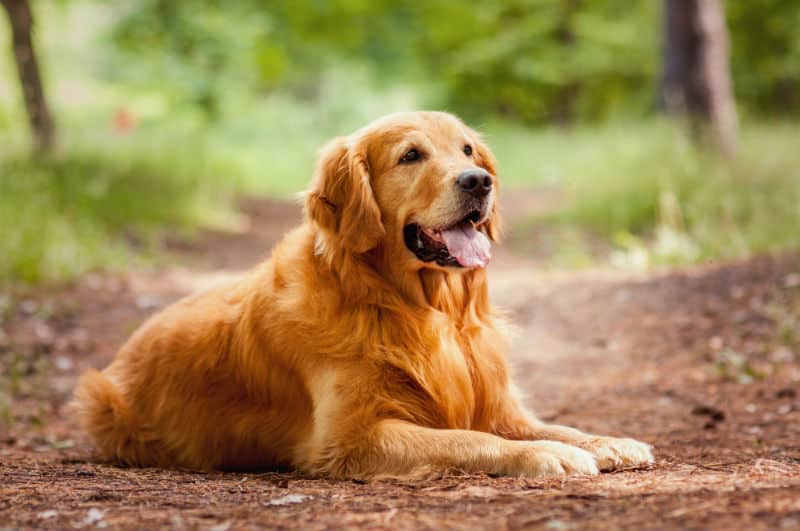
\includegraphics[width=0.5\textwidth]{exemplo-imagem.jpg}
    \legend{Fonte: \citeonline{citacao2}}
\end{figure}

Proin porta massa nec rutrum malesuada. Aliquam eget erat eu augue molestie malesuada scelerisque ac neque. Orci varius natoque penatibus et magnis dis parturient montes, nascetur ridiculus mus. Donec placerat ipsum sit amet felis sollicitudin feugiat. Maecenas mollis erat vel magna tincidunt, ut semper urna ultricies. In libero magna, maximus eget elit id, pulvinar pulvinar dolor. In hac habitasse platea dictumst. Suspendisse id felis iaculis, mattis velit a, pellentesque dui. Morbi interdum ante eu lorem egestas, a tempor erat vulputate. Curabitur eget nulla in odio dictum vestibulum. Praesent sodales dictum vestibulum. Vestibulum at justo consectetur, varius magna sed, pulvinar tortor. Duis sed varius nulla, non euismod eros. Proin iaculis turpis eget nibh volutpat pellentesque.

\citeonline{citacao3} exemplo de citação na mesma linha

Exemplo de lista de items sem enumeração:

 \begin{itemize}
    \item \textbf{item 1} exemplo de listagem.
    \item \textbf{item 2} exemplo de listagem.
    \item \textbf{item 3} exemplo de listagem.
 \end{itemize}

 Exemplo de lista de items com enumeração:

  \begin{enumerate}
    \item item 1
    \item item 2
    \item item 3
 \end{enumerate}

 Exemplo de equação:

 \begin{equation}
    P(A|B) = \frac{P(B|A)P(A)}{P(B)}
 \end{equation}

 \subsubsection{Subseção da subseção do capítulo de Revisão Bibliográfica}

 Exemplo de uso de tabela:

 \begin{table}[htb]
    \centering
    \caption{\label{resultL1knnEucli}Tabela de Exemplo}
    \begin{tabular}{ccc}
    \hline
    Dado 1 & Dado 2 & Dado 3\\ \hline
    Linha 1    & 0,000    & 0,000\\ \hline
    Linha 2    & ?        & 0,000\\ \hline
    Linha 3    & ?        & 0,000\\ \hline
    \end{tabular}
 \end{table}

% ========================================================================
% DESENVOLVIMENTO
% ========================================================================
 \chapter{Desenvolvimento}

 Lorem ipsum dolor sit amet, consectetur adipiscing elit. Sed sollicitudin tempor sapien in maximus. Quisque in vulputate dui, ac vestibulum sem. Suspendisse urna velit, dapibus nec egestas a, rhoncus vitae neque. Mauris quis efficitur augue. Aliquam quis tellus eget orci aliquet aliquam. Sed luctus, quam vitae elementum malesuada, quam lacus imperdiet urna, sed ullamcorper libero magna non elit. Cras laoreet arcu a augue volutpat, suscipit pretium tellus tempus. Sed eros tortor, imperdiet eu neque id, interdum egestas tortor.

% ========================================================================
% RESULTADOS
% ========================================================================
 \chapter{Resultados}

 Lorem ipsum dolor sit amet, consectetur adipiscing elit. Sed sollicitudin tempor sapien in maximus. Quisque in vulputate dui, ac vestibulum sem. Suspendisse urna velit, dapibus nec egestas a, rhoncus vitae neque. Mauris quis efficitur augue. Aliquam quis tellus eget orci aliquet aliquam. Sed luctus, quam vitae elementum malesuada, quam lacus imperdiet urna, sed ullamcorper libero magna non elit. Cras laoreet arcu a augue volutpat, suscipit pretium tellus tempus. Sed eros tortor, imperdiet eu neque id, interdum egestas tortor.

% ========================================================================
% CONCLUSÃO
% ========================================================================
 \chapter{Conclusão}

 Lorem ipsum dolor sit amet, consectetur adipiscing elit. Sed sollicitudin tempor sapien in maximus. Quisque in vulputate dui, ac vestibulum sem. Suspendisse urna velit, dapibus nec egestas a, rhoncus vitae neque. Mauris quis efficitur augue. Aliquam quis tellus eget orci aliquet aliquam. Sed luctus, quam vitae elementum malesuada, quam lacus imperdiet urna, sed ullamcorper libero magna non elit. Cras laoreet arcu a augue volutpat, suscipit pretium tellus tempus. Sed eros tortor, imperdiet eu neque id, interdum egestas tortor.

 \section{Trabalhos Futuros}

\begin{itemize}
    \item Trabalho Futuro 1
    \item Trabalho Futuro 2
    \item Trabalho Futuro 3
\end{itemize}

\postextual

% ========================================================================
% BIBLIOGRAFIA
% ========================================================================
\bibliography{bibliografia.bib}

% ========================================================================
% APENDICES
% ========================================================================
\begin{apendicesenv}

\partapendices

\chapter{\label{AnexoA}Exemplo de seção de anexo}

\begin{lstlisting}
EXEMPLO DE CODIGO A SER ADICIONADO
\end{lstlisting}

\end{apendicesenv}

\end{document}